\chapter{Literature Review}
\label{LitReview}

This chapter shall provide summaries of the background information required to understand the content of this thesis, and also review the state of the art of the various subjects that this thesis covers.

\section{Colour Science}

Organisms on earth posses visual systems such that they can glean information about spatially remote objects through the sensing of light reflected from these objects towards the organism. They are able to do this because the sun emits electromagnetic radiation (which we call `light' when it is within our visual sensitivity range), our atmosphere transmits many parts of this radiation (absorbing some wavelengths more so than others), and objects absorb some and reflect some of this radiation (again, some wavelengths more so than others), as shown in Figure \ref{fig:SPD}.
%minnaert?

\begin{figure}[hbtp]
\includegraphics[max width=\textwidth]{figs/LitRev/daylightAndBananas.pdf}
\caption{The \gls{SPD} of a single measurement of daylight (sunlight plus scattered blue-sky light, from \citet{hernandez-andres_color_2001}) and the light reflected from 2 different surfaces - a green banana and a yellow banana (data from personal correspondence with David Slaughter after \citet{li_optical_1997}), computed by multiplying the \gls{SPD} by the measured \glspl{SRF} of the two surfaces. \Glspl{SPD} normalised such that the max of the daylight \gls{SPD} is 1.}
\label{fig:SPD}
\end{figure}

Our perception of colour generally correlates with the way in which objects preferentially reflect some wavelengths over others (described by the \acrfull{SRF}) which assists in the recognition of objects (that's a banana) and the discrimination of distinct objects, often in a manner that is ecologically beneficial (that's a \emph{ripe} banana).

\newpage

\subsection{Colorimetry}

\textit{The current recommended source for colorimetry is \gls{CIE} document `\gls{CIE} 015:2018'\citep{cie_cie_2018}\footnote{Though as \citet{fairchild_cie_2019} notes, this document is `expensive and somewhat difficult to find', and as such I have been using a draft of the now superseded `\gls{CIE} 15.3:2004'\citep{cie_cie_2004-2} as my personal guide.}. Whlist this is the authoritative reference, my personal opinion is that an understanding of colorimetry of \gls{CIE} colorimetry is best gained from an understanding of it's history, and for this I recommend Janos Schanda's book `Colorimetry: Understanding the \gls{CIE} System'\citep{schanda_colorimetry_2007}.}

\bigskip

Colorimetry is the study of the quantitative specification of colour. As a subjective, internal and anthropocentric concept, in order to measure anything meaningful and comparable, we use a standard observer, or more precisely, one of a number of defined standard observers \cite{cie_bs_2011}.

The classic standard observer was defined by the \gls{CIE} in 1931, following experiments by Wright and Guild \cite{wright_re-determination_1929, guild_colorimetric_1931}. Despite several more recently published standard observers, the 1931 observer is still much used, and I shall use it in the following example of how a basic colorimetric computation is performed.

\glsreset{SPD}
\glsreset{SRF}
\glsreset{CMF}
\glsreset{SSF}

An illuminant is defined by its \gls{SPD}, a surface as it's \gls{SRF}, and a the sensitivity of a sensor (such as a photosensitive cell in the retina, or a pixel in a camera) by its \gls{CMF} (or in the case that biologically based measurements are used - the \gls{SSF}).

\begin{figure}[htbp]
\includegraphics[max width=\textwidth]{figs/LitRev/SPDetc.pdf}
\caption{An \gls{SPD} (D65), a set of \glspl{SRF} (from a Macbeth Colour Checker) and three \glspl{CMF} (\gls{CIE} 1931 observer).}
\label{fig:specFun}
\end{figure}
% % How is D65 normalised here?

The light reaching the eye for a given reflecting surface under a given illuminant (termed the `colour signal') can be computed by multiplying the \gls{SPD} by the \gls{SRF} at each sampled interval.

\begin{equation}
\phi(\lambda)=R(\lambda) \cdot S(\lambda)
\end{equation}

where $R(\lambda)$ is the \gls{SRF}, $R(\lambda)$ is the \gls{SPD} and $\phi(\lambda)$ is the resulting colour signal. From this a set of values termed `tristimulus values' may be computed. Tristimulus values are computed by multiplying the colour signal by the \glspl{CMF} or \glspl{SSF}, and following the principle of univariance (that each cone type cannot alone distinguish between different wavelengths) the tristimulus values can, to some extent, be thought of as containing the entirety of the chromatic information about a surface (excluding high level colour appearance phenomena predicted by \Glspl{CAM}, and properties such as gloss).

\begin{subequations}
\begin{align}
X=k \sum_{\lambda} \phi(\lambda) \overline{x}(\lambda) \Delta \lambda \\ 
Y=k \sum_{\lambda} \phi(\lambda) \overline{y}(\lambda) \Delta \lambda \\ 
Z=k \sum_{\lambda} \phi(\lambda) \overline{z}(\lambda) \Delta \lambda
\end{align}
\label{eq:XYZ}
\end{subequations}

\nopagebreak %this doesn't work currently

where $\overline{x}(\lambda)$ (said `x bar'), $\overline{y}(\lambda)$ and $\overline{z}(\lambda)$ are the \glspl{CMF} of the 1931 observer (or are replaced by the \Glspl{CMF}/\Glspl{SSF} or the chosen observer), $\phi(\lambda)$ is as defined above, $k$ is a normalising factor, and it is recommended that $\Delta\lambda$ be 1nm. It is traditional to set $k$ such that $Y=100$, though in the case of relative colorimetry (most cases) is often ignored since the following equation renders it superfluous.

From the tristimulus values chromaticity co-ordinates ($x$ and $y$) can be computed. These can then be plotted on a 1931 chromaticity space diagram, shown as Figure \ref{fig:1931}.

\begin{subequations}
\begin{align}
x=\frac{X}{X+Y+Z} \\
y=\frac{Y}{X+Y+Z} 
\end{align}
\label{eq:1931chrom}
\end{subequations}

% Here's a \gls{MATLAB} example, using \gls{PTB} for data:

% \begin{lstlisting}[language=MATLAB]
% load spd_D65 % SPD: CIE D-series illuminant D65
% load sur_macbeth % SRF: macbeth colour checker
% load T_xyz1931 % CMF: CIE 1931

% colourSignals = sur_macbeth.*spd_D65;
% XYZ = T_xyz1931*colourSignals;
% xy = [XYZ(1,:)./sum(XYZ);XYZ(2,:)./sum(XYZ)];
% \end{lstlisting}

% Plotting: 

% \begin{lstlisting}[language=MATLAB]
% spectralLocus = [T_xyz1931(1,:)./sum(T_xyz1931);T_xyz1931(2,:)./sum(T_xyz1931)];
% sRGBSpectralLocus = XYZToSRGBPrimary(T_xyz1931);

% figure, hold on, 
% scatter(spectralLocus(1,1:70),spectralLocus(2,1:70),[],sRGBSpectralLocus(:,1:70)','filled')
% scatter(xy(1,:),xy(2,:),'k')
% axis equal, axis([0 1 0 1])
% xticks([0 1]), yticks([0 1])
% xlabel('x'), ylabel('y')
% \end{lstlisting}

\begin{figure}[htbp]
\includegraphics[max width=\textwidth]{figs/LitRev/ColorimetryDemo1.pdf}
\caption{The \gls{CIE} 1931 chromaticity space, showing the chromaticity of the macbeth colour checker patches under D65. Note that for all of the plots in this section, the colours used for the spectral loci are only very rough approximations.}
\label{fig:1931}
\end{figure}

\subsubsection{Specific Colour Spaces}

Over time various other colour spaces have been proposed and formally accepted by the \gls{CIE}, each aiming to improve upon a prior space in one or more ways. One of the most frequently sought characteristics for a colour space is perceptual uniformity, whereby a set distance in one part of the space is comparable in terms of apparent colour difference to that same distance in another part of the space.

One such chromaticity space which shall be used extensively in this thesis is the \gls{CIE} 1976 UCS (uniform chromaticity scale) space, which is a relatively simple transformation of the 1931 chromaticity space. The conversion can be accomplished in a number of analogous fashions, one of which is shown below.

\begin{subequations}
\begin{align}
u' &= 4x / (-2x + 12y + 3) \\
v' &= 9y / (-2x + 12y + 3)
\end{align}
\end{subequations}

where $x$ and $y$ are the 1931 chromaticity co-ordinates as defined in Equation \ref{eq:1931chrom}. The data presented in Figure \ref{fig:1931} are re-plotted in this new space in Figure \ref{fig:UCS}.

\begin{figure}[htbp]
\includegraphics[max width=\textwidth]{figs/LitRev/ColorimetryDemo3.pdf}
\caption{\gls{CIE} 1976 UCS (uniform chromaticity scale) space, showing the chromaticity of the macbeth colour checker patches under D65 (as in Figure \ref{fig:1931}).}
\label{fig:UCS}
\end{figure}

A three-dimensional extension to the CIE 1976 UCS space is the \gls{CIE} 1976 L*u*v* colour space, often abbreviated to CIELUV, which aims to provide perceptual uniformity in a space that includes both chromaticity and lightness (relative to a white object under the same illumination). It is defined as follows:

\begin{subequations}
\begin{align}
L^{*} &= 116 f(Y/Y_{n})-16 \\
\textrm{where} f(Y/Y_{n}) &= (Y/Y_{n})^{1/3} &\textrm{ if } (Y/Y_{n}) > (24/116)^{3} \\
\textrm{or} f(Y/Y_{n}) &= (841/108)(Y/Y_{n})+16/116 &\textrm{ if } (Y/Y_{n}) \leq (24/116)^{3} \\
u^{*} &= 13L^{*}(u'-u'_{n}) \\ 
v^{*} &= 13L^{*}(v'-v'_{n})
\end{align}
\end{subequations}

where $Y_{n}$, $u'_{n}$ and $v'_{n}$ refer to the colour stimulus of a perfect reflector. The same data presented in Figures \ref{fig:1931} and \ref{fig:UCS} is presented in CIELUV in Figure \ref{fig:CIELUV} (though of course the three-dimensional quality of the data is somewhat lost).

\begin{figure}[htbp]
\includegraphics[max width=\textwidth]{figs/LitRev/ColorimetryDemo4.pdf}
\caption{A representation of CIELUV, showing the values for the macbeth colour checker patches under D65 (as in Figure \ref{fig:1931} and \ref{fig:UCS}). Note that if viewed from above, the distribution of points would appear similar to as in Figure \ref{fig:UCS}. If all of the points were of uniform L*, then the distribution would be identical, only with different scaling.}
\label{fig:CIELUV}
\end{figure}

Introduced at the same time as CIELUV was a colourspace with a similar goal of perceptual uniformity: CIELAB. They are similar in many ways, and share $L^{*}$ and if the CIE committee in charge of recommending such a space for adoption had been able to decide upon one or the other, one would have sufficed. As it is, both exist. CIELAB seems to be in slightly more common usage, but CIELUV is used in this thesis (particularly Chapter \ref{chap:Tablet}) due to the close link to an associated chromaticity space (the CIE 1976 UCS space). CIELAB is defined as follows:

\begin{subequations}
\begin{align}
L^{*} &= 116 f(Y/Y_{n})-16 \\
\textrm{where} f(Y/Y_{n}) &= (Y/Y_{n})^{1/3} &\textrm{ if } (Y/Y_{n}) > (24/116)^{3} \\
\textrm{or} f(Y/Y_{n}) &= (841/108)(Y/Y_{n})+16/116 &\textrm{ if } (Y/Y_{n}) \leq (24/116)^{3} \\
a^{*} &= 500[f(X/X_{n}) - f(Y/Y_{n})] \\ 
b^{*} &= 200[f(Y/Y_{n}) - f(Z/Z_{n})] \\
\end{align}
\end{subequations}

where $f(X/X_{n})$ and $f(Z/Z_{n})$ follow the same format as $f(X/X_{n})$.

The final colour space presented here is the \acrfull{MB} colour space. This space does not aspire to be perceptually uniform\footnote{This can be clearly noted by comparing Figure \ref{fig:lrMB} with previous figures. Where this set of chromaticities previously spanned the spaces fairly broadly, here all the chromaticities inhabit only a small portion of the chromaticity space.}. Instead, it aspires to provide a colour space which has a physiological underpinning. As such, the observer used consists of nominal \glspl{SSF} (rather than \glspl{CMF}), and the conversion from tristimulus values to chromaticity space attempts to mirror the way in which this actually occurs physiologically.

It was originally proposed by \citet{macleod_chromaticity_1979}, but was recently revised and endorsed by the \gls{CIE}, in documents `CIE 170-1:2006'\citep{cie_cie_2006} and `CIE 170-2:2015'\citep{cie_cie_2015}\footnote{I understand that the final publication in the series (`CIE 170-3:XXXX') is in preparation.}. The revisions included the definition of a new observer, based on the work of \citet{stockman_spectral_1999} and \citet{stockman_spectral_2000}, and the introduction of a set of new normalising terms, such that it is now calculated as follows.

\begin{subequations}
\begin{align}
L_{\text{MB}}&=k_{l} \sum_{\lambda} \phi(\lambda) \overline{l}(\lambda) \Delta \lambda \\ 
M_{\text{MB}}&=k_{m} \sum_{\lambda} \phi(\lambda) \overline{m}(\lambda) \Delta \lambda \\ 
S_{\text{MB}}&=k_{s} \sum_{\lambda} \phi(\lambda) \overline{s}(\lambda) \Delta \lambda
\end{align}
\label{eq:MBTristim}
\end{subequations}

where $k_{l}$ = 0.68990272, $k_{m}$ = 0.34832189, $k_{s}$ = 0.03715971. This set differs minimally but purposefully from Equation \ref{eq:XYZ}; in the choice of observer ($\overline{lms}$), and in the use of different scaling factors for each tristimulus value. \gls{MB} chromaticity values are then calculated as follows:

\begin{subequations}
\begin{align}
l_{\text{MB}}&= \frac{L_{\text{MB}}}{L_{\text{MB}}+M_{\text{MB}}} \\ 
s_{\text{MB}}&= \frac{S_{\text{MB}}}{L_{\text{MB}}+M_{\text{MB}}} 
\end{align}
\label{eq:MB}
\end{subequations}

Whereas the relationship between the axes of previous colour spaces was important, here the axes are nominally independent (representing different post-receptoral mechanisms) and so the scaling between the axes is arbitrary. The same data as presented previously is presented again in Figure \ref{fig:lrMB} in a \gls{MB} chromaticity space.

\begin{figure}[htbp]
\includegraphics[max width=\textwidth]{figs/LitRev/ColorimetryDemo5.pdf}
\caption{A \gls{MB} chromaticity space diagram (as per \gls{CIE} 170-2:2015\citep{cie_cie_2015}) showing the values for the macbeth colour checker patches under D65, as in previous figures.}
\label{fig:lrMB}
\end{figure}

\clearpage
\subsection{Colour rendering}

Colour rendering indices provide an indication of the colour appearance of objects under a test illumination. Colour fidelity indices (properly a subset of colour rendering indices, however the most commonly used colour rendering index is in fact a colour fidelity index) are designed to describe how well a light source will produce a faithful appearance in terms of corresponding colorimetry to an appearance under \gls{CIE} D-series illuminant (daylight proxy) or a black body radiator. %Target values are generally provided in museum lighting guidelines \citep{ies_ies_1996,druzik_guidelines_2012,cibse_lighting_2015,thomson_museum_1986}. The recommended value for the ubiquitously used \gls{CIE}~R\textsubscript{a} (As defined in \gls{CIE} 13.3:1995 \citep{cie_cie_1995}), often informally referred to as `CRI', varies from publication to publication, but is generally \gls{CIE}~R\textsubscript{a}$>$80, but with no experimental work referenced to support this figure. 
Research in colour rendering is at a point of change and development, with the recognition that a single figure might never be enough to describe the complex, multidimensional, subjective and context dependent qualia of colour rendering \citep{rea_color_2008}. Thus new indices, and modifications and addenda to long-established indices are being proposed \citep{smet_memory_2012,davis_color_2010,rea_practical_2010,ies_ies_2015,teunissen_characterising_2016}.

If we were to take a bunch of balloons (or any objects, but balloons provide a simple and vivid image) of varied and multiple colours, from an area lit with daylight to an area lit with artificial light, and the colour appearance changes, for example the colours become more dull, we would generally be disappointed. In this case, we could say that we were dissatisfied by the colour rendering qualities of the artificial light source. If the colours remained the same we probably would think little of it, but if we were pressed for a comment, we might say that the colour appearance was satisfactory. 

If the balloons stayed the same colour as they had been under daylight, we would be witnessing a high level of colour fidelity (fidelity meaning faithfulness or truthfulness). If fidelity aligns well with the priorities of the user, then high levels of fidelity are desirable. If the appearance of the balloons had changed in some other way than becoming more dull - for example the colours became more vivid or the hue of certain balloons changed drastically, we might not neccessarily be disappointed, but this would still represent a situation where we were witnessing poor fidelity.

Generally when discussing colour fidelity, we are actually discussing fidelity to appearance under daylight or sometimes a Planckian radiator, aka a black body radiator. This is a fine comparison, but one which should be consciously considered; fidelity is not a measure of a light source per se, it is a comparison of that light source to a reference illuminant.

Fidelity has long been considered semi-analogous for colour rendering as a whole, but it is really only one element of colour rendering\footnote{Here I should point out that the \gls{CIE} definition of colour rendering, from the publication \gls{CIE} S 017/E:2011 ILV: International Lighting Vocabulary \citep{cie_cie_2011} reads: ``Effect of an illuminant on the colour appearance of objects by conscious or subconscious comparison with their colour appearance under a reference illuminant.'' You might notice the similarities to the definition I have ascribed to colour fidelity, and specifically not colour rendering. This is an unfortunate clash of nomenclature which I see as inappropriate usage on the part of \gls{CIE}, and at some point I hope this official definition will be updated to match the modern vernacular.}. When considering how `good' a light source is at facilitating colour with the objects which it illuminates, we might consider different measures alongside or in place of fidelity.

\begin{itemize}
\item \emph{Colour Fidelity (to recap)} - A measure of comparison between how colours appear under daylight (or other reference) and how they appear under another light source. %Do the balloons appear the same colour indoors and out? Are individual colours important or is an average suitably representative?
\item \emph{Chromatic Discrimination} - The ability of a light source to illuminate objects such that subtle differences in colour are made most visible. %Can you tell the difference between all the balloons? How big are the differences? Are threshold differences more or less important than the perceived magnitude of suprathreshold differences?
\item \emph{Observer Preference} - Subjective preferences for the colour of objects, potentially related to an increase in saturation, or an observer's memory of colours, or specific colour effects (e.g. increased saturation of skin tones). %Do the balloons look `nicer'/more vivid/more like the last time you saw them?
\end{itemize}

These areas overlap, and often exhibit correlation. For example, if a light source has properties which allow for high fidelity rendering, quite often that light source might also allow for good colour discrimination and also facilitate colours which might appear natural and/or pleasing. These are not reliable correlations however; it is quite possible to have a light source with very dissimilar properties to daylight that could score highly on discrimination and/or preference, or vice versa.

The index in widest use currently for quantifying colour rendering is \gls{CIE}~R\textsubscript{a} (The General Colour Rendering Index). At the beginning of this doctoral project, this metric was used almost exclusively to generate the figure listed as `CRI' on the packaging for bulbs available commercially. %In the intervening time, \gls{IES} RP-30-15 \citep{ies_ies_2015}, and more recently \gls{IES} RP-30-18 \citep{ies_ies_2018}, have been published and have found considerable uptake from manufacturers.

\gls{CIE}~R\textsubscript{a} is a colour fidelity metric, produced by computing the colour differences of 8 specified \glspl{TCS}, between the situation where illumination is provided by the test source and that where it is provided by a reference illuminant with the same \gls{CCT} as the test source, and taking the arithmetic mean of these colour differences. The index is scaled such that the highest score is 100, for light sources which reproduce the \gls{TCS} set under the reference illuminant exactly, with any light source which induces a colour shift receiving a value less than 100, descending below 0 if the magnitude of the shifts are great enough.

The most recent version of the standard specifying this metric is `\gls{CIE} 13.3-1995 Method of Measuring and Specifying Colour Rendering Properties of Light Sources' \citep{cie_cie_1995}. This document briefly overviews the history of, and necessity for, a colour rendering index and highlights areas of the procedure which vary compared to previous recommendations, and clearly details the recommended procedure. The process is summarised in the flow chart of Figure \ref{fig:criflow}. For a worked example see \citet[p.388]{hunt_measuring_2011}.

In response to a lack of confidence that \gls{CIE}~R\textsubscript{a} delivered meaningful values for \gls{LED} illumination, a considerable amount of research and discussion has revolved around the subject of a colour rendering index to supersede \gls{CIE}~R\textsubscript{a}. This is commonly complicated by the incorrect assumption that the values obtained from a fidelity index in some way correlate with preference. A more valid criticism of \gls{CIE}~R\textsubscript{a} is that it comprises deprecated methods (for example, use of the \gls{CIE} 1960 UCS color space, now superseded) and data sets (a rather limited set of \glspl{TCS}, drawn from measurements of Munsell papers) for computing intermediary stages within the process of calculation, and thus this theoretically limits the `correctness' of any values produced by it.

Following many years where multiple \gls{CIE} technical committees aimed to deliver updated colour rendering indices, but subsequently didn't make any firm recommendations, an \gls{IES} group was formed with the aim of examining the issue. The output of this \gls{IES} group was the production of \gls{IES} TM-30-15\cite{ies_ies_2015}, which follows the same philosophy as \gls{CIE}~R\textsubscript{a} but with more modern colour science. It is still a contentious issue whether this updated index genuinely offers advantages over \gls{CIE}~R\textsubscript{a}. 
% it also includes a bunch of other things...
% and IES TM-30-18?

Alternative propositions which offer fundamentally different approaches to the evaluation of colour rendering have been offered in recent years, including: 
\begin{itemize}
\item indices based on production of memory colours \citep{smet_memory_2012}.
\item indices which consider the size of the gamut of a \gls{TCS} set \citep{rea_color_2008,teunissen_characterising_2016}.
\item indices which are fundamentally fidelity indices but which penalise or reward specific traits known to be disliked/preferred \citep{ohno_rationale_2010}.
\end{itemize}

\begin{figure}[htbp]
\includegraphics[max width=\textwidth]{figs/LitRev/criflow.png}
\caption{The stages of calculation for the computation of the \gls{CIE} General Colour Rendering Index. Notes: Reference illuminant: the same or nearly the same \gls{CCT}. Below 5000K reference spectrum will be that of a black body radiator, and from 5000K `one of a series of spectral power distributions of phases of daylight'.}
\label{fig:criflow}
\end{figure}

\clearpage

\subsection{Chromatic Adaptation and Colour Constancy}

\textit{Shortly after the start of my PhD program I attended a symposium for PhD students in the field of lighting research (LumeNet). At this symposium Prof. Michael Pointer delivered a welcome talk, and one particular part of it stuck with me.}

\textit{He described how at the start of his PhD studies \citep{pointer_colour_1972}, he had made copies of every paper which had been written on his subject (Chromatic Adaptation) which were available from the library, and written to any authors whose work he had been unable to access, requesting copies. At the end of his first year he had a binder which contained, as far as he was aware, everything ever written on the subject. He finished his story rather abruptly, along the lines of ``since then, so many people have written on the subject that it would take much longer than you have within a PhD program to read it all. I don't know what you all will do''. Not an encouraging thought!}

\textit{With this in mind, I shall attempt only to cover the basics and a few select papers of particular relevance in the following section, and shall take this opportunity to note my debt to a number of comprehensive overview papers, book chapters and theses on this subject: \citet{foster_color_2011,maloney_computational_1984,barnard_practical_1999,smithson_sensory_2005,hurlbert_computational_1998,brainard_color_2014,fairchild_color_2013}.}

\subsubsection{The problem}

At the start of this section I stated that ``Our perception of colour generally correlates with the way in which objects preferentially reflect some wavelengths over others''. It transpires that this ability is non-trivial, because our visual systems do not have access to the \glspl{SRF} of the objects which are seen, only the levels to which retinal cells are excited, which depends on the interaction of illuminant, surface and sensor. 

Figure \ref{fig:problem} demonstrates the problem, by reproducing Figure \ref{fig:1931} with a minor adjustment; where the previous figure had the chromaticities of the set of surfaces under only a single illuminant, a large number of illuminants are used here. It can be seen that it is not uncommon for one surface to have a chromaticity under one illuminant that another surface has under a different illuminant. Thus, the relationship between surface and chromaticity appears to break down.

\begin{figure}[htbp]
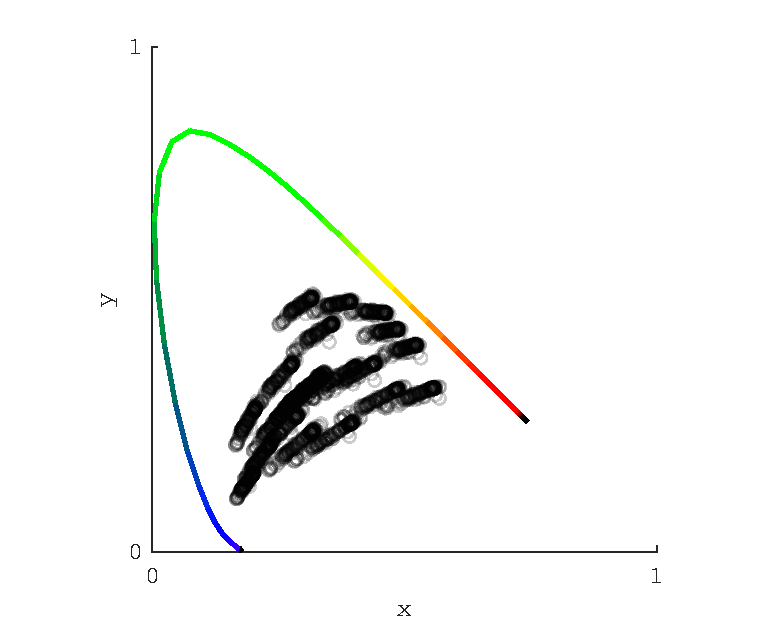
\includegraphics[max width=\textwidth]{figs/LitRev/ColorimetryDemo6.pdf}
\caption{A reproduction of Figure \ref{fig:1931}, but this time with the chromaticity co-ordinates for the 24 macbeth colour checker patches under a range of daylights, drawn from the Granada dataset \citep{hernandez-andres_color_2001} (further described in Section \ref{sec:coldata}).}
\label{fig:problem}
\end{figure}

In order to provide a representation of colour where the perceived colour remains constant across changes in illuminant (thus the term \emph{colour constancy}), the human visual system must find a way to solve this problem.

\subsubsection{Adaptation}

`Adaptation' is the general mechanism by which a finite range of sensitivity can be shifted within absolute sensitivity bounds. The benefit of having an adaptive system, as opposed to a fixed system, is that the sensitivity of the system to small changes is maximised, whilst maintaining a broad overall sensitivity, at the expense of being able to sense over the entire range at a single time-point. A visual demonstration of this is shown in Figure \ref{fig:Valeton} where it can be seen that that at a single level of adaptation (a single line) the range of intensity over which responses are generated is relatively small, but is extended through adaptation.

\begin{figure}[htbp]
\includegraphics[max width=\textwidth]{figs/LitRev/Valeton.png}
\caption{Cone flash response at different levels of adaptation in macaques, reproduced from \citet{valeton_light_1983}. On the left `DA' stands for dark-adapted, with the rising numbers for the other lines relating to rising adapting levels.}
\label{fig:Valeton}
\end{figure}

In an environment such as the terrestrial environment, there is a great range in the level of illumination, but this range is rarely existent contiguously; levels of illumination tend to be similar across a scene, and only change rather slowly over time. The notable exception, and thus where we notice the expense of having an adaptive visual system, comes when we enter or exit an environment where illumination is almost entirely excluded, such as a dark cave or below-decks of a boat. 

Where the process of adaptation responds to overall illumination levels, it is referred to as light adaptation and dark adaptation. Where the process of adaptation responds to the wavelength composition of light reaching the eye it is referred to as chromatic adaptation.

In a natural environment, a change in the wavelength composition of radiation reaching the eye from a specific object might be caused by changing weather or time of day, or by the physical movement of the object from one space to another (where different lighting exists in the two different spaces). Figure \ref{fig:SPDnorm} shows a set of measured daylight \glspl{SPD}, normalised by luminance, showing that the wavelength composition varies quite considerably, though in a relatively systematic fashion.

\begin{figure}[htbp]
\includegraphics[max width=\textwidth]{figs/LitRev/ColorimetryDemo7.pdf}
\caption{The \glspl{SPD} of a subset of the daylight measurements of \citet{hernandez-andres_color_2001} (further described in Section \ref{sec:coldata}), normalised by luminance.}
\label{fig:SPDnorm}
\end{figure}

\subsubsection{Mechanistic vs. Inferential}

In the literature there seems to be a long-running grapple between colour constancy and chromatic adaptation, with blurred boundaries and mixed definitions occurring frequently. \citet{brill_chromatic_1986} drive a wedge between the two concepts, but refute the traditional division that chromatic adaptation is the process and colour constancy is the ability, asserting that the two should be considered as separate processes, operating on different timescales and in different fashions.

\citet{hurlbert_computational_1998} divides computational models of colour constancy into two classes: \emph{sensory} and \emph{perceptual}, which broadly follow the low-level / high-level divide. `Sensory' models `could be achieved early in visual processing by adaptive scaling of the initial receptor responses'. `Perceptual' models `would necessarily occur at later stages of visual processing'.

Hurlbert [personal communication] notes that understanding the differing perspectives of researchers from different fields allows one to understand how the mixed use of these terms in the literature may have arisen: 

\begin{itquote}{}
The mixed use of the terms chromatic adaptation and colour constancy is largely explained by different usages in different fields. In \emph{colour science}, chromatic adaptation is often considered synonymous with colour constancy, as it is considered to be the only mechanism contributing to stabilising colour appearance under changes in illumination. In \emph{vision science}, colour constancy is generally defined as a perceptual phenomenon, and distinction is made between different contributory mechanisms at different levels (which \citet{hurlbert_computational_1998} attempts to define and onto which different proposed computational solutions are mapped).
\end{itquote}

Within vision science, the most common use of the term `chromatic adaptation' now seems to be to refer to low level adaptation, with \citet{brainard_color_2014} using the term `mechanistic' to refer to this type of transformation.

\begin{itquote}
Adaptation of this sort supports constancy to the extent that its overall effect is to stabilize the post-receptoral representation of the light reflected from objects across changes of illumination (as well as other contextual changes).
\end{itquote}

The term `colour constancy', by contrast, is used to refer to higher level inference-based processes, which occur at faster timescales than are possible by adaptation alone \citep{rinner_time_2000}. It seems likely that multiple processes work in tandem at multiple levels and timescales to achieve colour constancy \citep{hurlbert_colour_2007}.



\subsubsection{Von Kries Adaptation}

The conceptually simplest model of chromatic adaptation, and the forefather of many other models, is that referred to as Von Kries adaptation.

Johannes von Kries was one of the first to deeply consider chromatic adaptation, and appears to have understood it as a problem of sensory adaptation. In his formative series of papers, available in translation \citep{von_kries_beitrag_1970}, he laid out how the study of chromatic adaptation could be divided into two broad and complementary aims. 

The first referred to the systematic representation of the transforms in sensation caused by specific adaptations, such that \textit{``for any light mixture stimulating the readapted part [of the retina], another light mixture is specified that stimulates the same sensation in a normally adapted part \dots The purpose of this study would be solved completely if a general rule could be obtained for the effects of all possible adaptions.''} The search for `corresponding colours' (pairs of colours which match under asymmetric adaptation states), and for suitable systems to predict the appearance of colours in all situations, fall within this category of exploration. Out of this aim grew the study of \glspl{CAT}, where the search for an algorithm which would mathematically predict the locations in colour space of corresponding colours has been the fundamental goal \citep{cie_tc_1-52_cie_2004}.

Von Kries suggested that the second categorical aim of chromatic adaptation research ought to be to discover `how the adaptation is produced by exposure to any particular color, continued over an extended period of time.' 

Von Kries' distinction carves a divide between the study of the mechanisms of chromatic adaptation, and the effects of chromatic adaptation. It would be unreasonable to think of these areas of study as unrelated, but it seems reasonable to recognise their separability. 

%In the same set series of papers, von Kries laid out his understanding of chromatic adaptation, in terms of both how corresponding colours might be calculated, and how one might consider the underlying mechanisms which allow for colour constancy to operate. Here I shall abridge some of his writings to present the most salient insights, and attempt to explain what is meant by a `von Kries transform' in modern parlance.

Von Kries noted that `light mixtures that appear matched to the white-adapted eye always remain matched to the eye when it is adapted in any other manner.' This is known to be only partly true; if referring to photopic vision solely (where rods are bleached and cones provide the basis for vision). The implication of this statement is that the spectral sensitivities of the cone cells do not change as a result of chromatic adaptation. If they were to change in some way, then distinct mixtures of light which match in one adaptive state might fail to match under a different state. Von Kries referred to this idea as the `persistence rule.'

The second rule which von Kries presents is referred to as the `theorem of proportionality'. This theorem claims that when two pairs of corresponding colours (colours A and B under illuminant 1, and colours C and D under illuminant 2) are additively combined (A with B, and C with D), the resulting colours will also be corresponding colours. It follows from the von Kries' theorem of proportionality that increasing or decreasing the luminance of corresponding stimuli shouldn't void their equality, though of course this statement relies even more heavily on the caveat that this should only be assumed for photopic vision.

Von Kries goes on to suggest that it also follows that, if considered in combination with Grassmann's law \citep{grassmann_zur_1853}, the conversion of any arbitrary light by exposure to conditions causing a specific chromatic adaptation can be known if the nature of three other conversions are known. This relies on it being possible to consider any light as a linear combination of three others, and for the mechanism of chromatic adaptation to depend solely on the fatiguing of three independent systems.

Von Kries' assertions may be mathematically described as:

\begin{subequations}
\begin{align}
L_{a}&=K_{L}L \\
M_{a}&=K_{M}M \\
S_{a}&=K_{S}S
\end{align}
\end{subequations}

where $L$, $M$ and $S$ represent the cone group responses; $K_{L}$, $K_{M}$ and $K_{S}$ represent distinct scalars and $L_{a}$, $M_{a}$ and $S_{a}$ represent the post adaptation cone group responses\footnote{This specific notation is taken from \citet[p. 183]{fairchild_color_2013}.}. In terms of what might set these scalars, or gain values, von Kries suggested that: 

\begin{itquote}{von_kries_beitrag_1970}
the organ of vision becomes less effective for that kind or for that part of its performance which is demanded from it for an extended period of time, whereas it becomes more effective for the activity which is, in a sense, opposed to that. This can be conceived in the sense that the individual components present in the organ of vision are completely independent of one another and each is fatigued or adapted exclusively according to its own function.
\end{itquote}

Many interpretations have been made of this statement, and a corresponding number of nominations for methods by which to calculate values of $K$ have been proposed. The most frequently considered methods are those referred to as \acrfull{GW} (where the reciprocal of the mean response across a scene is used) and \acrfull{BiW} (where the reciprocal of the brightest point in the scene is used). \citet{finlayson_shades_2004} showed that these two variants can be considered as part of a single framework (Minkowski norm), and that other members of this family of algorithms provide benefits over \gls{GW} and \gls{BiW}.

Von Kries' thoughts have inspired many decades of research into \glspl{CAT}, which are a vital part of modern colour appearance models and other colour science computations, such as colour rendering index calculations. This relatively simple concept has remained relevant, as noted by \citet[p. 182]{fairchild_color_2013} who reproduces this quote:

\begin{citequote}{von_kries_beitrag_1970}
If some day it becomes possible to distinguish in an objective way the
various effects of light by direct observation of the retina, people will perhaps
recall with pitying smiles the efforts of previous decades which
undertook to seek an understanding of the same phenomena by such
lengthy detours.
\end{citequote}

followed by the comment:

\begin{citequote}{fairchild_color_2013}
Over eleven decades later, there is no one looking back at von Kries’ work
with a “pitying smile.” Rather, many are looking back at his work with
astonishment at how well it has withstood the test of time.
\end{citequote}

\subsubsection{Retinex}

Considered in the context on von Kries' work, the Retinex model of Land et al. \citep{land_retinex_1964,land_lightness_1971,land_recent_1983,land_recent_1986,mccann_quantitative_1976} might be described as `Von Kries adaptation with spatial considerations' but I imagine such a statement would have rather riled the often bombastic sounding Land. It appears to have been Land's understanding that the Retinex model was not a model of chromatic adaptation, but rather a model to usurp and do away with the very concept of chromatic adaptation (Land's papers on the subject \citep{land_retinex_1964,land_lightness_1971,land_recent_1983,land_recent_1986} do not once use the term `chromatic adaptation', nor is the work of von Kries ever explicitly referred to). 

Land was fond of picking apart Newton's statements regarding colour; particularly that the perception of colour was the result of an objects' `excess and predominance in the [spectra of the] reflected light' \citep{newton_opticks_1704}. Land asserted that rather than work from the premise that the visual system was correcting an absolute record of the world, by normalising it to account for the ambient light source, one should instead consider visual input only as a relative record, where each element within a scene only takes on properties by comparison with the other elements of the scene. 

He suggested for consideration the idea of the human visual system recording three separate lightness images, each representing the recording from a different band of receptors, where each element within each image is scaled against the brightest element in each specific image. Retinex theory also provides an interesting algorithm for discounting not only coloured illumination but illumination which varies across the visual field.

However, \citet{barnard_practical_1999} points out that the various versions of the Retinex algorithm simplify to versions of the Von Kries adaptation, and \citet{brainard_analysis_1986} found that `the algorithm is too sensitive to changes in the color of nearby objects to serve as an adequate model of human color constancy'. In addition, it has been found to be computationally difficult to implement, with no clear way in which it could be biologically implemented (though see \citet{hurlbert_formal_1986}).

The work of Land et al. has spurred a great deal of progress in the world of digital imaging, where the term `computational colour constancy' is used. The number of distinct algorithms increases at a rate which seems to always accelerate, and I shall not review them all here, though I shall point to valuable overview papers:  \citet{hordley_reevaluation_2006, gijsenij_computational_2011, hurlbert_computational_1998}.

\subsubsection{Linear models}

If we extend the common interpretation of colour constancy (that colours should remain constant), to a stricter case where we actively try to recover the \glspl{SRF} of surfaces, simple Von Kries-type transformations no longer suffice. \citet{maloney_physics-based_2001} and \citet{yang_illuminant_2001} discuss what they term the `RGB heuristic'. Simply put - this is the commonly held assumption that a set of cone catches under one illuminant will be related to a second set of cone catches under another by a transformation which can be fully described by the chromaticities of the illuminants. As \citet{maloney_physics-based_2001} says `there is no \emph{mathematical} reason to expect [this] to hold, even approximately'. This can be considered from the perspective of colour rendering; it is known that objects which are metamers under one illuminant might not be under another. This renders simple models of colour constancy ineffective. \citet{foster_frequency_2006} quantified the frequency of metamerism in real scenes and found it to be `sufficiently large to affect visual inferences about material identity'.

For this stricter definition of colour constancy Maloney et al. \citep{maloney_computational_1984, maloney_color_1986} propose a method which makes use of discrete linear models, whereby the set of real \glspl{SRF} and real \glspl{SPD} are approximated by a small number of fixed basis functions. 

\citet{maloney_color_1986} find that `with three classes of photoreceptors, we can exactly recover surface reflectances drawn from a fixed model of surface reflectance with at most two degrees of freedom'. \citet{maloney_computational_1984} showed that this generalised such that with $n$ classes of photoreceptors, \glspl{SRF} could be reconstructed for surfaces drawn from models with $n-1$ degrees of freedom, so long as there were not more than $n$ degrees of freedom in the illumination model, and so long as the minimum complexity condition was met (there were enough surfaces visible).

Despite its mathematical elegance, quantitative analysis of this algorithm showed that its performance was poor \cite{brainard_bayesian_1994, finlayson_color_1995}, which is not surprising considering that natural surface \glspl{SRF} generally require more than two basis functions for accurate reconstruction.

\bigskip

There are many further ideas, theories, and concepts relating to colour constancy and chromatic adaptation which are beyond the scope of this chapter, but that the reader may find of interest: gamut mapping algorithms \citep{forsyth_colour_1990,forsyth_novel_1990,forsyth_colour_1989,finlayson_color_1996}, bayesian colour constancy \citep{finlayson_color_2001, brainard_bayesian_2006,gazzaniga_bayesian_2009, brainard_bayesian_1994,gehler_bayesian_2008} and specular-reflectance-based algorithms \citep{mollon_monge_2006, morimoto_discrimination_2018,hurlbert_computational_1998}.

%% Removed stuff ---------------------------------


%Colour constancy refers to the stable perception of object colour appearance, in spite of a change in illumination which would cause a change in the nature of the stimuli reaching an observer\footnote{The terms `chromatic adaptation' and `colour constancy' are often used interchangeably; within this thesis I shall use `chromatic adaptation' to refer to an adaptive mechanism, and `colour constancy' as the ability possessed by an organism. For a discussion of the distinction of chromatic adaptation and colour constancy see \citet{brill_chromatic_1986}}. This objective change in stimuli seems to be effectively but not completely discounted by the human visual system; in order to maintain a stable perception of object appearance. 

%If however, one asked an observer whether the \emph{appearance} of an object has changed between the two conditions, the observer would generally say that it has. To some extent, we seem to have access to both the `raw input signals' and some estimate of the underlying \gls{SRF}.


%It is the popular understanding that when the illumination changes, the colour of an object (to use the term `colour' in its vernacular form, as representing an object attribute) does not change. This understanding holds true for all but the most extreme artificial illuminations, such as very narrow-band illuminantion. 


% \begin{figure}[htbp]
% \includegraphics[max width=\textwidth]{figs/LitRev/fosterflowers.png}
% \caption{A single scene under two illuminants (\Gls{CCT} = 4000k and 25000K), reproduced from \citet{foster_color_2011}.}
% \label{fig:fosterflowers}
% \end{figure}

% \begin{figure}[htbp]
% \includegraphics[max width=\textwidth]{figs/LitRev/greyballs.png}
% \caption{Reproduced from \citet{nascimento_spatial_2014}. Original figure caption: ``The color rendition on the left shows the scene with six embedded probe spheres indicated by numbers. The dot plot [on the right] shows the distribution of the CCTs of the local illumination at the 17 sample points on each of the spheres.''}
% \label{fig:greyballs}
% \end{figure}

%Figure \ref{fig:greyballs} gives an indication of the extent to which an object (or more precisely in this case, a group of nominally identical objects) can have varying colorimetric attributes across relatively minor spatial variation. 
%KC: This reads oddly to me, as it's more the illuminance that's varying than the object (if I've understood?).  I'd rephrase this.

% \begin{figure}[htbp]
% \includegraphics[max width=\textwidth]{figs/LitRev/X.png}
% \caption{\hl{Figure showing variation over time.}}
% \label{fig:X}
% \end{figure}

% Figure \ref{fig:fosterflowers} shows a single scene under illumination of two different \glspl{CCT}. The appearance of the object under the two illuminants is likely to have remained somewhat stable to an observer within the real scene, with observers choosing similar colour names for the object under each condition\footnote{Of course the appearance here, with these two images side-by-side, highlights the differences between the two conditions, and shows that under a single state of adaptation there is a clear distinction.}. 


% \subsubsection{Can chromatic adaptation fully account for colour constancy?}

% It may at first appear as though chromatic adaptation may be able to fully account for colour constancy

% RGB heuristic
% yes - cornsweet
% mechanistic vs inferential


% A similar level of variation occurs across time, for example as the sun passes behind a cloud.

% And so we have the central problem of colour constancy and chromatic adaptation: objects of which we have stable colour perceptions are able to be variant in both radiometric and colorimetric attributes without losing their apparent stability. The study of colour constancy aims to answer many questions which revolve around this central conundrum.

% Traditionally %(pre-1986, when \citet{arend_simultaneous_1986} performed what \citet{foster_color_2011} refers to as `the first systematic behavioral experiments' on color constancy) 
% there have existed two stances regards the nature of colour constancy; one held that it was enabled by adaptation of the sensory system, and the other that it was the result of unconscious inference. %KC: citation required
% It is my understanding that whilst great progress has been made in the intervening three decades, this is still a central question, although it appears to be widely accepted that the two frameworks might be complementary rather than mutually exclusive. %KC: citation required

%The best justification for their separation is perhaps that success in their study might serve different aims. 
%The first, the prediction of colour appearance, serves to further the utility of colour science, in particular colour appearance modelling, and the other systems which rely upon colour appearance modelling, such as colour difference formulation. 
%The second is best considered a vision science problem, concerned as it is with the function of the human visual organ, and advancement might endow us with an extension in our understanding of the human body. This in turn would have benefit in multiple areas, including feeding back to the prior aim, for once we understand the underlying mechanics we stand a much better chance of creating robust predictors of colour appearance. 
%Of particular interest to this author, understanding the underlying mechanisms of colour constancy should allow for a more intelligent design of lighting for the spaces which we inhabit, considering that artificial lighting need only resemble natural lighting to the extent that the visual system treats it as similar enough. Creating a colorimetric match to a specific spectra such as D65 is relatively easy, but until chromatic adaptation is more thoroughly understood it is not necessarily entirely clear what the appearance of such a match, or objects illuminated by it, might be. 

%The investigation of \glspl{CAT} generally occurs through the fitting of algorithms to data of corresponding colours, collected in varying manners, such that corresponding colours might be predicted for specific situations. The principal divides between the types of \gls{CAT} tend to hinge upon the method used to collect the data. \citet{nayatani_development_2006} divides the set as those derived from chromatic adaptation theory and those derived from fitting to experimental data, whereas Luo44 makes the divide between those studies based on aperture based experimental procedures and non-aperture based experimental procedures (which generally incorporate more complex, and therefore arguably more realistic, stimuli). Both parties use the terms `CAT Type I/II' to refer to these distinctions, but it is not entirely clear whether their distinctions are complementary. 

% This duality %get rid of this bollocks
% is mirrored by Foster37 in his discussion of the experimental methods employed in colour constancy research where he describes fundamental differences between those experiments which probe chromatic adaptation by asking observers to make `paper matches' (make it look like these two patches were cut from the same sheet of paper) and h/s/b matches (where observers are asked to match appearance in a non-relational manner, that is to match the qualia of a stimuli). This duality occurs again in Foster's37 comparison of relational and non-relational colour constancy, where relational refers to the maintaining of colour relationships in a scene and non-relational again refers to abstracted stimuli qualia). It is my suspicion that all of these disparate dualities are representations of the fundamental duality considered at the beginning of this chapter; that of a distinction between sensory adaptation and inferential computation.

\subsection{Experimental Methods for Colour Constancy Research}

\begin{citequote}{hurlbert_colour_2007}
\emph{How is colour constancy measured?} With difficulty.
\end{citequote}


\hl{A large range of experimental methods have been used to investigate the problem of colour constancy \dots} % partly because different experimenters were approaching the problem from different angles aiming to accomplish subtly separate goals.
% Those approaching from a mathematical angle (perhaps with the mind-set `if we find the algorithm which predicts corresponding colours a- this is very useful for industry and b- we can then work backwards to explain how human colour constancy may occur') are concerned primarily with producing chromatic adaptation transforms.
% Those approaching colour constancy with a basic interest in the physiology and general function of colour constancy have adopted/created a rather wider set of experimental techniques, owing to the fact that this direction of study is much less well defined than the former, and is at a more exploratory stage of its development.
% The \gls{CIE} TC 1-52 report (\gls{CIE} 160:200442) includes an interesting note on the distinction between these two broad approaches; an appendix discusses the reasons why a concerted recommendation was not reached by the group lists the principal factor being a distinction between perspectives as described above. 
% \gls{CIE} TC 1-5242 and Luo44 provide a comprehensive overview of the different methods which have been used by the CAT group:
% 1.	Haploscopic matching
% 2.	Local Adaptation Matching
% 3.	Memory Matching
% 4.	Magnitude Estimation
% Haploscopic Matching is the most common technique in this field, and the term refers to experiments which differentially adapt the two eyes and allow an observer to vary attributes of the stimulus presented to one eye such that it in some way matches the attributes of a fixed stimulus shown to another eye. Whilst this is in many ways unnatural, the benefits are that an experiment can be set up so that there is no time interference (the presentations are simultaneous, so memory effects are avoided) and that high precision of match is relatively easily achieved. As assumption is made that the adaptation of each eye is independent.
 
% Figure 11 From42.
% Local Adaptation Matching can be considered as a variation of haploscopic matching where instead of differing adaptational stimuli being presented to each eye, differing adaptational stimuli are presented to different parts of the same eye (spatially distinct areas of the same retina). The assumption here is that there is minimal intra-retinal interaction. MacAdam's 1956 study49 epitomises this technique. This experimental technique requires that observers minimise eye movement, in order to maintain spatially distinct adaptation.
% Memory Matching has traditionally been performed by training observers to communicate colour sensation through the munsell system notation50,51, and then asking observers adapted to different ambient lighting to describe set real objects using such notation. This technique is not much used due to many limitations and confounding factors. Luo44 details the limitations  of this experimental technique succinctly: `a substantial training period being required, complicated procedures for data analysis, lower precision than that of haploscopic technique, limited capacity for retaining information, and memory distortion.'
% Magnitude Estimation appears to be similar to memory matching, in that observers are requested to verbally describe an object whilst in an ambient adapting field. The distinction is that the observers are requested to communicate their perceptions using the perceptually meaningful attributes of hue, saturation and brightness, and as such results can be easily integrated into colour appearance models. Recent experiments52,53,54,55,56,57 collected data which was used to create CIECAM97s.
% Away from the development of CATs, a subtly different set of experimental techniques has been developed with which to probe the operation of colour constancy. An admirable overview is provided by Foster37:
% 1.	Asymmetric Matching
% 2.	Colour Naming
% 3.	Achromatic Adjustment
% 4.	Discriminating Illuminant Changes from Reflectance Changes
% Asymmetric matching is in many ways synonymous to the haploscopic matching described above and by in \gls{CIE} 160:200442, in that it describes an experimental set-up whereby one stimuli is compared with another, generally where each stimuli exists within a distinct adapting field and attributes of one stimuli can be either adjusted or responded to by an observer. The term asymmetric matching might be thought to be inclusive of a wider range of experimental set-ups, where haploscopic (Greek roots: haploieides, single and skopeo, to view) is necessarily concerned with each individual eye receiving distinct input. Asymmetric matching may refer to experiments where stimuli are viewed simultaneously, successively, or in an alternating fashion, binocularly or haploscopically.
% Colour Naming is a technique employed with the aim being a more natural task than  asymmetric matching, and removing some of the `instruction effects' probed by Arend and Reeves40. Foster argues37 that colour naming represents a task apt to measure colour constancy more directly, as opposed to the `relational colour constancy' often studied in asymmetric matching experiments, since it concerns identification rather than equivalence. One clear benefit seems to be that the observer needn't be aware of the equivalence; it is expected that in such experiments there will be only one stimulus, perhaps with a temporally variant adapting field. An observer is simply asked to name colours, and this should theoretically result in a measure of adaptational colour constancy as opposed to inferential colour constancy, so long as the stimuli is suitably abstract . Colour names may be of a fixed set, or an observer may be given free choice. Analysis of results can employ a naming centroid based approach or a boundary focused approach. Speigle and Brainard58 proposed a novel approach combining magnitude estimation and colour naming with the aim to improve precision of response.
% Achromatic Adjustment experiments ask an observer to in some way set a stimulus to a neutral achromatic tone, on the assumption that the internal grey point of an observer shifts in response to different adapting fields. These adjustments are generally easy for an observer to make, but the extrapolation of the results makes various assumptions about conceptual colour space and the nature of achromacy. Experiments are easily confounded by complex or real stimuli where there exists a close-to-neutral object in the scene which could consciously or unconsciously be used as a reference.
% Discriminating illuminant changes from reflectance changes provides a key way to examine colour constancy in an operational manner. Following the assumption that chromatic adaptation allows an observer to discount the illuminant in some manner, an experimental set up where observers are requested to distinguish between an illuminant change and a reflectance change represents a situation which very closely mirrors the natural process of colour constancy. This experimental technique is well placed to examine whether or not colour constancy in this form is active and efficient, but it provides little way of probing the underlying mechanisms of colour constancy.

% %recent advances in colour constancy?
% % using more realistic stimuli
% % the grey edges algo
% % the comparison of grey edge and grey world/bright is white

\subsection{Intrinsically Photosensitive Retinal Ganglion Cells (ipRGCs)}

\textit{A recent review by \citet{spitschan_melanopsin_2019} provides an overview of this rapidly progressing research area.}

\bigskip

Retinal rod and cone cells (of three types, l/m/s) are well established as the primary receptors for human vision, and their connections and properties are relatively well understood. Two distinct signalling pathways originate from the retina, one which is associated with image formation and the other which is considered to be \gls{NIF}, and which influences systems such as circadian rhythm entrainment, pupillary reflex and melatonin release. It was originally thought that rods and cones were the sole inputs to both of these pathways\citep{hankins_melanopsin_2008}.

\Glspl{RGC} combine signals from groups of cones and rods and relay these signals via the optic nerve to the lateral geniculate nucleus, which in turn processes and relays them further to the cortex for additional processing, allowing for classical vision of objects, movement and colour. \Glspl{ipRGC} are a sub-class of retinal ganglion cells, which in addition to combining and relaying signals exhibit some intrinsic photosensitivity of their own. 

This intrinsic photosenstivity was only confirmed recently\citep{qiu_induction_2005} relative to our knowledge of other retinal cell types, following a search for a retinal cell type or combination of cell types which would fit the spectral sensitivity properties found to influence entraining the circadian rhythm in humans and other animals\citep{brainard_human_2001,brainard_action_2001}, which was dissimilar to all of the spectral sensitivities of the cell classes known at the time.

Additionally, it was found that animals and humans with no functioning cones or rods were still able to have a correctly functioning circadian system\citep{freedman_regulation_1999,zaidi_short-wavelength_2007}, further suggesting that that the circadian rhythm was influenced by a novel receptor with a distinct photoreceptor. It is now believed to be these cells which provide input to the second of the signalling pathways originating in the retina, that which controls the \gls{NIF} response to illumination.

\Glspl{ipRGC} were found to express a photopigment fitting such attributes, named melanopsin. The spectral sensitivity of melanopsin peaks around 480nm\citep{qiu_induction_2005,hankins_primary_2002,dacey_melanopsin-expressing_2005,peirson_melanopsin_2006,bailes_human_2013} which places it between the s-cone (cyanolabe photopsin) and rod cell (rhodopic rhodopsin) peak spectral sensitivities%, see Figure \ref{fig:specsens}
. In humans, pre-receptoral filtering leads to a functional peak sensitivity of closer to 490nm\citep{cie_cie_2015-1}. There is uncertainty regarding the potential bistable nature of melanopsin, and whether this would have a functional effect on the spectral sensitivity of melanopsin\citep{cie_cie_2015-1,mure_melanopsin_2009,rollag_does_2008}.

\Glspl{ipRGC} are sparse in the retina; discounting input from other cell types, they operate at a much lower resolution than as would be required for meaningful spatial vision. They also operate much more slowly compared to other cell types, taking several seconds to respond, but are able to sustain a response in contrast to other retinal cell types which are able to respond quickly but only for short periods.

It has been proposed that \glspl{ipRGC} may allow an observer to sense a level of absolute irradiance\citep{brown_melanopsin_2010}. 

\subsubsection{The image-forming role of ipRGCs}

In recent years there has been a large number of publications examining the role of melanopsin outside of \gls{NIF} vision.

Spatial:
\cite{ecker_melanopsin-expressing_2010}
\cite{spitschan_vision_2017}
\cite{mouland_responses_2017}
\cite{allen_melanopsin_2017}
\cite{allen_form_2019}

Colour:
\cite{cao_evidence_2018}
\cite{spitschan_human_2017-1}
\cite{zele_melanopsin_2018}

\section{Museum Lighting}

\bigskip

\begin{quote}
`Museums and art galleries collect, preserve, and display natural artifacts and/or examples of human achievement and analyze their impact on the world and the universe around us. Effective exhibit lighting must balance exhibition and conservation needs and enrich the museum experience.'
\end{quote}

\begin{flushright}IES RP-30-96 Museum and Art Gallery Lighting: \\A Recommended Practice \citep{ies_ies_1996}\end{flushright}

\bigskip

Lighting in museums is required to satisfy multiple criteria; perhaps the least contestable requirement being that the lighting illuminate objects such that they are suitably visible to museum visitors. Also of utmost importance in most museum settings is that the lighting does not have an unreasonably damaging effect upon the objects or environment, be this through direct photodegradation or as a result of heat transfer. Further to these requirements, an increased or optimal visual quality is generally desirable, although what this represents or how to achieve it is generally ambiguous.

In sweeping terms, all electromagnetic radiation (visible and non-visible) damages objects, and more radiation damages objects proportionally moreso. Thus the question becomes: \emph{how little light can we use to illuminate objects such that they're visible to the extent required?} The inverse form, sometimes used on the assumption that more light always represents an increase in observer satisfaction/pleasure is: \emph{`how much light can we use so that only $x$ damage occurs over $y$ time'}. 

Industry guidance documents provide advice on how to manage lighting to best address the above requirements and many other additional specific requirements through the recommendation of procedure and provision of target figures for quantitative variables. \Gls{UV} radiation, being of no visual benefit but having potential to harm, is now excluded from gallery spaces as an industry standard.

\subsection{Damage functions} \label{sec:DamageIndex}

\textit{The key reference on this subject is CIE 157:2004 \citep{cie_cie_2004}, and valuable talks on the subject were given at the recent Museum Lighting Symposium \& Workshops\citep{pokorska_book_2017} (which the author helped to organise), and have been made freely available online\footnote{See in particular the talks by David Saunders (\url{https://www.youtube.com/watch?v=H4d0qH0IBcI&t}) and Stefan Michalski (\url{https://www.youtube.com/watch?v=XUY9biLQqlw})}.}.

\bigskip

In heritage science `damage functions' are ``functions of unacceptable change, dependent on agents of change''\citep{strlic_damage_2013}. The goal of damage functions in heritage lighting engineering is to give a quantitative means by which to predict the amount of damage caused to a prototypical object by a given light source, and to assist in limiting such damage. They generally follow the logic that radiation of lower wavelength is likely to cause more damage to objects.

\citet{harrison_report_1953} is generally acknowledged as the first to suggest such a function, but he himself acknowledges that it had ``long been established that the shorter the wavelength (visible yellow, green, blue, violet and invisible UV being progressively shorter) the more photochemically potent will be such radiant energy, provided such energy is actually absorbed''. \citet[p.9]{harrison_report_1953} defined the `radiation hazard associated with a light source' as:

\begin{equation}
    \sum_{0}^{\infty} \mathrm{H}_{\lambda} \mathrm{D}_{\lambda} \Delta \lambda / \sum_{0}^{\infty} \mathrm{H}_{\lambda} \overline{\mathrm{y}}_{\lambda} \Delta \lambda
    \label{eq:Harrison}
\end{equation}

where $\mathrm{H}_{\lambda}$ is the spectral irradiance, $\mathrm{D}_{\lambda}$ is the `Relative Damage Factor' (which is extrapolated from the data collected shortly prior to Harrison's own report by the National Bureau of Standards \citep{national_bureau_of_standards_preservation_1951}, and shown in Figure \ref{fig:Harrison}), and $\overline{\mathrm{y}}_{\lambda}$ is the CIE 1924 photopic $V_{\lambda}$ luminosity function. The resulting value would describe the amount of damage expected from a light source, normalised by its luminance.

\begin{figure}[htbp]
\includegraphics[max width=\textwidth]{figs/LitRev/HarrisonInd.pdf}
\caption{Harrison's \citep{harrison_report_1953} damage function ($\mathrm{D}_{\lambda}$), and luminous efficacy ($\overline{\mathrm{y}}_{\lambda}$), alongside the Declaration of Independence data \citep{national_bureau_of_standards_preservation_1951} from which it was extrapolated (re-normalised to match scale).}
\label{fig:Harrison}
\end{figure}

\begin{figure}[htbp]
\includegraphics[max width=\textwidth]{figs/LitRev/Saunders.pdf}
\caption{Graph courtesy of David Saunders, presented at the Museum Lighting Symposium \& Workshops \citep[p.61]{pokorska_book_2017} showing the relationship between wavelength and the bonds which can be broken in various molecules, with `Wavelength (nm)' on the abscissa and `Bond energy (kJ/mol)' on the ordinate.}
\label{fig:Saunders}
\end{figure}

There has been extended scepticism about the utility of damage functions in general, with the argument being that no one damage function could represent the vast range and complexities of real materials. \citet[p. 178]{thomson_museum_1978} wrote that ``for more fugitive materials \dots the figure for visible radiation would be higher. On the other hand \dots the fastest dyes are probably affected only by UV. Thus it can be seen that no single figure can be given for damage versus wavelength''.

Criticism was aimed at this specific damage function due to it's derivation from such a small and minimally representative dataset - Harrison's data was `extended' from the 5 datapoints measured by the National Bureau of Standards \citep{national_bureau_of_standards_preservation_1951} in their investigations of how to best care for the Declaration of Independence\footnote{It is a curiosity that these minimal figures would not in fact have been much use to those planning the care for the declaration, since in the report it is noted that ``The deterioration of animal parchment is not as rapid as that of the low-grade paper for which the damage factors were determined''\citep{national_bureau_of_standards_preservation_1951}, and the Declaration of Independence is written on animal parchment.}, and was derived from the study of `low-grade paper', which cannot to said to represent the average museum item\footnote{Though \emph{no} material truly can!}.

CIE 157:2004 \citep{cie_cie_2004} notes that whilst Harrison's proposal failed to gain acceptance as the procedure for comparing the damage potential of different types of light sources, it did convince people of the ills of \gls{UV}, with the result that daylight was subsequently eliminated from many galleries.

Following \citet{cuttle_lighting_1988}, who noted that Harrison's damage function could be well fit by an inverted logarithmic function, with parameters controlling the slope and normalisation point of the function, CIE 157:2004 provided the following equation:

\begin{equation}
    s(\lambda)_{\mathrm{dm,rel}}=\exp [-b(\lambda-n)]
    \label{eq:damfac}
\end{equation}

where differing values of $b$ for 5 categories of item are provided (Table \ref{tab:b}), $n$ is the normalisation value (CIE 157:2004 uses a value of 300), and the $s(\lambda)_{\mathrm{dm,rel}}$ function is the estimated action spectrum for each category. $s(\lambda)_{\mathrm{dm,rel}}$ would be substituted into Equation \ref{eq:Harrison} for $\mathrm{D}_{\lambda}$. CIE 157:2004 also provides values of $H_{s,dm}$ which indicate the susceptibility of each group of materials to damage (where damage is considered as colour change%in $\Delta E_{\mathrm{ab}}^{\ast}$
).

\begin{table}[htbp]
\centering
\begin{tabular}{|c|l|l|l|}
\hline
Group & Samples & $H_{s,dm}$ (W h/m$^{2}$) & $b$ \\ \hline
a & Low-grade paper & 5 & 0.038 \\ \hline
b & Rag paper & 1200 & 0.0125 \\ \hline
c & Oil paints on canvas & 850 & 0.0115 \\ \hline
d & Textiles & 290 & 0.0100 \\ \hline
e & Water colours on rag paper & 175 & 0.0115 \\ \hline
\end{tabular}
\caption{Table reproduced from CIE 157:2004 \citep{cie_cie_2004}, showing the values for $H_{s,dm}$ and $b$ for various categories. Note: the source for this data is not particularly clear; it is listed as `The Berlin researchers', which is assumed to follow the references: \citet{krochmann_beleuchtung_1988,cie_cie_1991,hilbert_zur_1991}; none of which I have been able to access.}
\label{tab:b}
\end{table}

The more general criticism that damage functions will never be able to represent all museum objects is a valid concern, and can be well illustrated with the following logic: museums own objects of many different colours, different colours arise from different reflectance properties, different refelctance properties mean different wavelengths are absobed, and damage can only occur when radiation is absorbed. Thus it follows that one would expect two objects of different colours to have different damage functions. 

The classic study on how reflectance properties relate to damage is that of \citet{saunders_wavelength-dependent_1994}. They exposed a number of pigments to a range of wavelengths and measured the resulting damage. \citet{cuttle_control_1999} later replotted the data from this study (reproduced in Figure \ref{fig:Cuttle}), highlighting the apparent joint contributions of spectral reflectance and a general damage function to the individual damage functions. CIE 157:2004 notes however that this correspondence is not perfect or easily modellable, and that ``a workable system for characterising action spectra for colorants, including pigments and dyes, remains an unattained goal``. Recent studied have added new data (see esp. \citet{villmann_wavelength_2018}), and it is hoped that a general understanding may at some point be reached.

\begin{figure}[htbp]
\includegraphics[max width=\textwidth]{figs/LitRev/Cuttle.pdf}
\caption{Figure of \citet{cuttle_control_1999}, using data from \citet{saunders_wavelength-dependent_1994}, and reproduced here from CIE 157:2004 \citep{cie_cie_2004}.}
\label{fig:Cuttle}
\end{figure}

However, it is the opinion of this author that this argument is an exercise in artificial futility; whilst we may not be able to model the individual damage functions for every object in a museum, we may at least use one which has some bearing on the damage function, rather than the one which is implicitly used by museums currently - the CIE 1924 luminosity function ($\overline{\mathrm{y}}_{\lambda}$ of Figure \ref{fig:Harrison}), which relates to the sensitivity of the human eye rather than any type of object. \citet{cuttle_lighting_1988} puts it well: ``The argument, then, is not whether we have a [damage] function which is correct, but whether we can improve usefully upon the likely reliability of the present system''.
% See xxx

In the case where specific objects/pigments of interest can be identified, and their individual damage functions calculated, there is valuable recent research to draw on regarding methods for optimising light sources to minimise damage \citep{durmus_optimising_2017,durmus_colour_2015,durmus_optimising_2015,durmus_object_2017}.

With modern computation, and access to datasets, it becomes relatively easy to calculate a value of \Gls{DI}. Figure \ref{fig:Houser} shows the results for such computations for 401 illuminants and light sources (as per Equation \ref{eq:Harrison}, using a damage factor computed as per Equation \ref{eq:damfac}, but further normalised such that Illuminant A has a reference value of 1)\footnote{The code to reproduce this is available from: \url{https://github.com/da5nsy/DamageIndex}}. It can be seen that whilst most illuminants cluster around 1 there is a broad range. It should be remembered that these illuminants would in no way indicate their relative damage index to an observer or a purchaser, unless one went to the effort to look up or measure the \gls{SPD} and compute the damage factor. A careful or careless choice in this respect could easily double or halve the amount of time an item could be exhibited before succumbing to terminal damage.

\begin{figure}[htbp]
\includegraphics[max width=\textwidth]{figs/LitRev/DI.pdf}
\caption{The values of $DI$ for the 401 illuminants used by \citet{houser_review_2013}, available via \gls{PTB} as `spd\_houser', normalised such that \gls{CIE} Illuminant A receives a reference value of 1.}
\label{fig:Houser}
\end{figure}

\subsection{Interviews with Museum Professionals} \label{sec:Interviews}

\textit{The following work has been published as \textbf{`How is museum lighting selected? An insight into current practice in UK museums'} \citep{garside_how_2017}. An overview is presented here, focusing on the elements relevant to the rest of the thesis, rather than as an independent chapter.}

\medskip

In order to gain an understanding of how museum professionals currently specify lighting, interviews were conducted with 12 museum professionals representing 10 UK based museums, galleries or historic property management groups, in spring of 2016. A small number of these professionals represented UK-wide groups, but the majority represented London based institutions.

The interviews were semi-structured around a set of questions composed by the author and their academic supervisors (reproduced in \citet{garside_how_2017}). The choice to conduct these interviews in a semi-structured format as opposed to a fully-structured one was based on the desire to allow unanticipated topics to enter the conversation, so as to limit the potential for important subjects to be neglected due to naivety of foresight. The conversational format of the interviews meant that the resulting data was qualitative rather than quantitative, which to an extent hinders comparison, but it was decided that the variety of job roles and institutional sizes, and the small sample size, already made quantitative comparison of limited meaningfulness for this investigation.

The interviewees were contacted through introductions from supervisors, personal connections, or cold emails. Almost all held conservation based roles (the exception being an `exhibitions manager') and noted that their principal responsibility regards lighting was controlling the safety of lighting regards its ability to cause damage to the objects held and displayed by their respective institutions. This generally involved monitoring and analysis of existing lighting systems and natural illumination, creating general guidance documents for the specification of lighting in their specific institutions and for loan items, and providing guidance and recommendations for the fitting out of new galleries or gallery refits. Few considered themselves directly responsible for the appearance of museum objects, considering this to be a creative decision outside of their remits. Future work considering the perspective of others involved in museum lighting, such as representatives from external lighting design companies, is required.

Whilst a small number considered themselves active in the area of lighting research, all interviewees were responsible for more conservation considerations aside from lighting, limiting the practicable level of specialisation. Many considered communication and dissemination a key part of their role, often noting they often found themselves in the position of needing to educate other teams within their institution on subjects including lighting. 

\begin{quote}
``This is not my science, my job is pulling it out and presenting it to others.''
\end{quote}

Asked what each considered to be `good lighting', responses included `safe', `invisible' (you don't notice it), and `lighting which is appropriate for your objects and your exhibition' (noting the variability of requirements dependent on the particular object(s) being presented). Asked to present a list or range of priorities, many focused on the safety requirements of lighting. The principal safety concern for lighting was that it fell below specific illuminance criteria, dependent on the assumed sensitivity category of the object in question. The specific target values were generally those provided by \citet{thomson_museum_1986} of 50lx for sensitive items and 200lx for less sensitive items (which are based on the visual preference work of \citet{loe_preferred_1982}).

Considering a scale of other priorities, following the requirement for appropriate lux levels, considerations included: limiting/excluding \gls{UV}, obtaining an acceptable \gls{CRI} value, and time and capital costs associating with fitting and maintenance. Energy efficiency was also a driver, but this did not seem to be a factor within technology category, rather it was noted that many institutions are switching to \gls{LED} because of increased efficiency, but that the difference in efficiency between one \gls{LED} type and another was negligible compared to the saving in contrast to lighting technology which \gls{LED} was replacing, which was often tungsten.

The range of roles played in the procurement of lighting varied amongst those interviewed. Whilst some created guidance documents which would then be passed on to estates teams and exhibition designers or lighting designers specifically, others had a much more hands-on role, testing specific lighting before installation or making recommendations on a case-by-case basis. It was noted that whilst relamping and retrofitting was generally handled by `in house' teams, where new galleries or large temporary exhibitions were created it was common for an external lighting design company to be contracted to perform the work. When asked whether recommendations were normally followed, the general reply was that recommendations for lux exposure and UV content were almost always followed, but other recommendations (such as for \gls{CRI} or \gls{CCT}) were more loosely interpreted. In many cases recommendations for \gls{CCT} were not made.

When asked about the tools used to make such recommendations and choices, responses included references to guidelines and reference sources (most often \citet{thomson_museum_1986}, though also \citet{druzik_guidelines_2012} and \citet{british_standards_institution_pas_2012}), references to specific units such as `lux' used in tandem with recommendations from guidelines such as above, indices such as the \gls{CIE} general colour rendering index R$_a$ (referred ubiquitously to as `\gls{CRI}' by interviewees) and notes of specific conferences which were attended in order to stay up to date with the research on the subject. There was a general feeling that the current climate was one of swift technological change in lighting, which created an increased difficulty in staying up to date with developments. It was noted that attending conferences and industry workshops were very beneficial in assisting professionals to stay up to date. 

\begin{quote}
`   Things are moving so quickly that to rely on books which have taken two years to produce [does not suffice, because] things have moved on. Books (plus journals) used to be the main reference. Now things are moving at such a rapid pace.''
\end{quote}

A range of techniques were used to qualify whether specific lighting was `safe' or not. The most common practical technique was spot metering of lux values incident on specific objects, and selective dimming to drop incident lighting to the desired lux level in response to this. Some larger institutions with access to microfading equipment were able to use this in the determination of sensitivity of specific objects. One interviewee provided details of a spectral power distribution based method for considering the safety specifically of phosphor based \gls{LED} illumination, whereby the height of the blue peak was compared to the height of the peak of the broader peak above 500nm, and if the former was more than three times the height of the latter, that lighting was singled out as potentially not safe. Other interviewees had heard of this criteria, and some used it as a rough guide, but one remarked that it was `fairly arbitrary'. One of the most succinct and perhaps astute responses was ``what is `safe'?''. One interviewee referred to the website of \citet{padfield_relative_2012} where considerations for the `RE\%' (`relative spectral sensitivity normalised exposure values'), using the damage functions described by \citet{aydinli_deterioration_1990} are used.

The interviewees generally did not consider characteristics of the displayed objects such as geometry of illumination, broadly considering this to be the remit of a lighting designer or exhibition designer rather than a conservator.

One of the most interesting, and perhaps surprising findings was the ubiquity of visual testing of lighting, generally performed prior to any large installation. For relamping, manufacturer supplied attribute values were generally relied upon as this required less time/effort and was cheaper. The most common procedure for new installations seemed to be for an informal and minimal visual test to occur before widespread installation. In a single case however, visual testing was actively avoided (on the basis that visual testing could not deliver meaningful insights where the aim was accurate rendering as opposed to visually pleasing rendering) and in another case large scale visual testing was performed, including many different types/brands of lamp and a large number of museum staff, and a final decision was made almost entirely on the results of this testing.

\Glspl{LED} are now used, at least in part, in all the institutions involved in this survey. In several they are the primary lighting technology but in a small number they are used sparingly, only in applications such as the lighting of text information panels. In one they are used in a particularly minimal fashion, although this was attributed to the fact that the museum is moving location in the near future and thus capital investments in building infrastructure were being avoided for the present time. There was no one specific brand or type which seemed to be ubiquitous across institutions, rather each institution appeared to have relationships with different manufacturers and suppliers.

Most interviewees were aware of warnings which had been issued and well publicised in the mainstream press \citep{lewis_smith_will_2013} regards the potential of \gls{LED} sources to be especially degrading for specific objects. Interviewees saw these warnings as controversial and likely unwarranted, and were confident that research had been conducted which cleared \Glspl{LED} of causing an unacceptable level of damage in comparison with alternative technologies. When asked how they might assess a light source for safety, most replied that safety was assessed solely through use of an illuminance meter and lux targets, not through analysis of the \gls{SPD} or any other lighting attribute. Those who did critically assess the \gls{SPD} generally used no specific tools to do so, focusing attention on the wavelength of the spectral emission peak.

\begin{quote}
``We never normally adjust the lighting type for a given artwork, we adjust the intensity''
\end{quote}

\begin{quote}
``For all lighting we measure the \gls{SPD}, and check it is reasonable''
\end{quote}

They key driver behind the adoption of \Glspl{LED} appears to be energy efficiency increases and energy use reductions, as required by institution-wide directives, or as part of applications for planning permission. Secondary to this consideration, benefits noted include: decreased maintenance costs from extended lifetime of products, and a lack of availability of traditional bulbs, sometimes due to specific legislation which has in effect phased out some traditional technologies. One element holding back some interviewees from further investment was a residual feeling that this new technology was not yet fully proven. Many pointed out that the claims made regards extended lifetime of \Glspl{LED} were yet to be proven in real world environments due to the relatively new nature of the technology. Some also noted the high costs associated with having to change the underlying lighting infrastructure, where retrofitting wasn't possible or appropriate. A final note on this section - some interviewees were unsure about the ability of \Glspl{LED} to remain colour stable over the long expected lifetime of the products.

Interviewees reported that visitors had not generally responded to any changes in lighting technology, and this was taken to mean that any switch to \gls{LED} had not been negatively received. It was inconclusive whether or not the technology was positively received however. This could be a meaningful avenue for future work. In terms of the professionals own opinions of \gls{LED} lighting, all seemed favourable, though it was unclear how much of this effect was caused by extraneous or related effects such as a placebo effect due to the excitement of new technology, or different chromaticities or brightnesses of replacement technologies.  

\begin{quote}
``I like what I've seen. The galleries where we have just \gls{LED} spots, I feel happier. I went to [another institution, with abundant \gls{LED} lighting], I really like the galleries where they had \gls{LED} lighting, and it was more of a gut feeling rather than something which I could put my finger on, but actually, it felt cleaner to me.''
\end{quote}

Whilst all interviewees were interested in the idea of making objects appear brighter whilst reducing the level of damage caused, the point was made that whilst spectral tuning might benefit a prototypical object, it will not necessarily benefit real objects in real environments. It was also noted that the use of lux in making decisions was particularly problematic here, where varying the location of a blue peak could easily increase the level of damage but reduce the lux value.
Most interviewees had a basic understanding of colour temperature, and a limited understanding of chromatic adaptation. The colour temperature of lighting was generally not seen as a conservation issue (though there were exceptions to this), and rather as a creative consideration. One interviewee noted that it was manipulated to great effect by external lighting designers in order to create specific effects or atmosphere.

The justification for \gls{CCT} specification values generally appears to stem from two routes. Firstly, from guidance documents such as those provided by The Getty and the Canadian Conservation Institute \citep{druzik_guidelines_2012}, and secondly from a desire to match existing lighting, either daylight or more commonly tungsten (at around 3000K). It was rarely considered as a means to control damage, or as a way to enhance visual appearance, by those interviewed. One interviewee referred to the work of \citet{kruithof_tubular_1941} and \citet{scuello_museum_2004,scuello_museum_2004-1} as justification for choosing low \gls{CCT} illumination similar to tungsten. No specific issues relating to colour temperature were raised by interviewees.

The interviewees were very interested in the subject of accurate representation, and almost all seemed to regard accurate object representation as a key priority. The figures for R$_a$ quoted in internal documents at each institution were either 80, 85 or 90, as a minimum figure. In one institution, an R$_w$ value was calculated for each proposed light source (the R value of the test colour sample with the colour shift of greatest magnitude, aka `worst') and a cut-off of 80 imposed. However, most interviewees seemed unsure of the practical relevance of R$_a$, with many considering it a rough guideline which would be considered secondarily to a visual inspection of lighting.

Those who were particularly interested in the subject gave the impression that whilst the subject was considered philosophically in great detail, the tool which was actually used to analyse the colour rendering of a light source was still generally just R$_a$. A few interviewees were aware of TM-30-15 \citep{color_metric_task_group_of_the_ies_ies_2015}, and whilst it was respected, it was questioned whether it represented a real improvement over R$_a$.
On the subject of lighting philosophy, the opinions encountered generally aligned with the mechanics of R$_a$. That is to say; given a choice between illuminating an object such that it was beautified, visually restored (to a previous condition) or simply presented as it would appear under daylight/tungsten illumination, most opted for the final option. Whilst there was clear interest in the other options, and other creative ways in which to consider colour rendering, it was generally believed that the role of the museum should be to represent objects in an un-biased manner, and thus a fidelity index was an appropriate tool for discussing a light source's colour rendering properties. In the case where specialist lighting was used to special effect, the opinion was noted that \textit{`you have to be very clear about what you are doing and why'} in order to maintain the reputation of the museum as an arena for honest and unbiased representation.

Generally, the interviewees believed that visitor requirements were being met (although there is often difficulty in defining exactly what visitor requirements actually are) and no specific tool or technology was proposed that would provide a clear benefit. Several interviewees mentioned that a way to improve the accessibility of colour rendering indices (in terms of the ease with which they could be understood and applied) would be appreciated.

No interviewees knew of recent surveys similar to the present one.

\subsection{Visitor Requirements of Museum Lighting}

The visitor requirements of museum lighting are varied and complex. The examination and definition of these requirements has been the subject of a small number of studies, principally by \citet{kesner_museum_1993-1} in the USA in the early nineteen-nineties \citep{kesner_museum_1993,kesner_exhibition_1992,kesner_current_1991,kesner_analysis_1997}. These studies were based on survey based self-reporting, and concluded that colour accuracy was the highest requirement and that `richness' of colour was the lowest priority\footnote{A cautious interpretation of these results is advised, considering that there were high average scores for each category}.

\begin{quote}
Artifact appearance, particularly clarity of artefact form and accuracy of artifact color, is the most important visitor need. Although visual impression, specifically acceptable gallery brightness and rich artefact color, is least important among the factors, it too rated highly important \citep{kesner_museum_1993-1}.
\end{quote}

Further studies, spurred by recent adoption of \gls{LED} technology have been completed, although with very limited and questionably scientific basis at the Field Museum \citep{myer_demonstration_2010}.

Additionally work has been completed which describes the results of a written survey of museum professionals on the subject of lighting specification, focusing on SSL (effectively \gls{LED}) adoption, and their justification for specifying specific lighting \citep{perrin_ssl_2014}. 979 people who had requested access to the guidelines document produced by some of the same authors \citep{druzik_guidelines_2012} were emailed with a request for participation. 46 (4.7\%) responded with a completed survey. Of those, 30\% are described as `international' which considering the base of the authors is in the USA we can assume as meaning `not based in the USA'. The survey was prepared as part of the USA government's GATEWAY program, and can be considered as a follow-up to work on recommendations for specification \citep{druzik_guidelines_2012}. 

\noindent
The headline results are as follows:
\begin{itemize}
    \item When the `success' of new \gls{LED} based lighting schemes was evaluated the public reaction was either neutral or positive in all cases \footnote{There appears to be an issue with the data for this question however, with the `no response' garnering 48\% of the responses and `favorable response' garnering 55\%\dots}
    \item The distribution of staff response was broadly similar: `no response'-17\%, `negative response'-3\%, `favorable response'-80\%.
    \item The results of two priority ranking questions\footnote{`Rank the following lighting goals' and `Please rank the following factors in your selection of lamps'} are broadly similar:
    \begin{itemize}
        \item First question: The first priority is identified as `limiting damage' with other priorities broadly equal.
        \item Second question: Joint first priorities are identified as `colour and spectral power distribution' and `damage potential' with others broadly similar (though dimming, input power and warranty lagging behind others)
    \end{itemize}
    \item 91\% of respondents reported using `\gls{CRI}' which is assumed to refer to \gls{CIE} R$_a$. 6\% state that they refer to other Ri values, and 20\% report using CQS (Color Quality Scale \citep{ohno_rationale_2010,davis_color_2010}).
    \item 60\% of respondents report that they consider \gls{CCT}.
\end{itemize} 

\subsection{Museum Lighting Specification Guidance Documents}

Following the interviews with the museum professionals, the five most referred-to museum lighting guidance documents were reviewed, and a summary is presented here.

\noindent
The guidelines chosen for review were:
\begin{itemize}
\item The Museum Environment \citep{thomson_museum_1986}
\item \gls{CIE} 157:2004 Control of Damage to Museum Objects by Optical Radiation \citep{cie_cie_2004}
\item Guidelines for Selecting Solid-State Lighting for Museums \citep{druzik_guidelines_2012}
\item SLL LG8: Lighting for museums and art galleries \citep{cibse_lighting_2015}
\item IES RP-30-96 Museum and Art Gallery Lighting: A Recommended Practice \citep{ies_ies_1996}\footnote{This has since been usurped by \citet{illuminating_engineering_society_ies_2017}.}.
\end{itemize}

\noindent
In summary:
\begin{itemize}
\item Recommended values were provided for:
\begin{itemize}
\item \emph{Lux}: various, dependent on sensitivity, generally based on figures from the study of visual preference by \citet{loe_preferred_1982}.
\item \emph{R$_a$}: various, most frequently \textgreater 80, with no experimental basis referenced.
\item \emph{\gls{CCT}}: various, based implicitly on \citet{kruithof_tubular_1941} or on such ideas found empirically.
\end{itemize}
\item Most also suggested visual inspection as a valid means of assessment.
\item There was often blurring between recommendations concerned with visual appearance and those concerned with conservation. 
\end{itemize}

\subsection{CCT in museums}

\acrfull{CCT} describes the chromaticity of a light source on a one dimensional axis roughly from blue to yellow, based on the apparent chromaticity of a black body radiator at differing temperatures. It is often described as an important variable in museum lighting but definite recommendations, in the rare cases that they are given, are generally based on very general rules that predict that damage potential will be decreased if \gls{CCT} is minimised \citep{cie_cie_2004}, nostalgia for the appearance of tungsten lighting or questionable research on human preference \citep{kruithof_tubular_1941,fotios_revised_2017}. Whilst some research appears to have found optimal \glspl{CCT} for viewing artwork \citep{nascimento_best_2014,pinto_correlated_2008,scuello_museum_2004,scuello_museum_2004-1, liu_cultural_2013} results often have large inter-observer variability, context dependency and it is not uncommon for the headline findings of separate studies to be in contradiction. 

Specifications often refer implicitly or explicitly to the findings of \citet{kruithof_tubular_1941}, who found that at lower levels of illumination, lower \glspl{CCT} were preferred, and that at higher levels of illumination higher \glspl{CCT} were preferred. Whilst this general trend seems to have anecdotal support, it is possible that there may be lighting-technology-based confounds, and recently researchers \citep{vienot_kruithofs_2009} (including a meta-study of multiple other examinations \citep{fotios_revised_2017}) found there to be no provable correlation between preference and colour temperature.

The \gls{CIE} however, published a report showing the varying the \gls{CCT} of museum lighting could have a clear impact on the potential damage undergone by museum objects \citep{cie_cie_2004}. 

\begin{figure}[hbtp]
\includegraphics[max width=\textwidth]{figs/LitRev/CIE2004.png} 
\caption{Figure reproduced from CIE 157:2004 \citep[p.16]{cie_cie_2004}, showing the relationship between \gls{CCT} and relative damage potential.}
\label{fig:CIE2004}
\end{figure}

This research relies heavily upon the applicability of damage functions to the specific materials in question. Many (my supervisors) think that damage functions are no good because they're too general, but I would be cautious about throwing the baby out with the bathwater.

\begin{enumerate}
    \item They're the best that we have.
    \item We need something with general applicability anyway - I don't see anyone providing tailored lighting for every object which exists.
    \item The physics checks out.
    \item They're definitely applicable to at least some objects.
\end{enumerate}

To verify the findings of the \gls{CIE}, to extend their findings to \glspl{LED}, and to provide code for others to do similar research or even test their own lights/materials, I wrote some code\footnote{\url{https://github.com/da5nsy/DamageIndex/blob/c7851e27ca1b0915013d8723db04704b49b4085e/CalcDI.m}} which would calculate a \gls{DI}. Then I used that code to compute a new version of the \gls{CIE} plot.

%\afterpage{\clearpage}
%\includepdf[pages=-,rotate=90, offset=75 -75]{figs/LitRev/CCTvsDI.pdf}
% \begin{figure}[t]
%     \caption{The \glspl{CCT} and \glspl{DI} of the \glspl{SPD} used by \citet{houser_review_2013} [provided via personal communication, but now partially available via \gls{PTB} as `spd\_houser'].}
%     \label{fig:CCTvsDI}
% \end{figure} 

\begin{fullpagefigure}
\figpdf[pages=-,rotate=90, offset=75 -75]{figs/LitRev/CCTvsDI.pdf}
\caption{The \glspl{CCT} and \glspl{DI} of the \glspl{SPD} used by \citet{houser_review_2013} [provided via personal communication, but now partially available via \gls{PTB} as `spd\_houser'].}
\label{fig:CCTvsDI}
\end{fullpagefigure}

The results of these computations show a clear relationship between \gls{CCT} and \gls{DI}. Considering that this is not currently taken advantage of in museum lighting, it seems as though there is a great potential for reducing damage whilst maintaining visitor visual satisfaction.

\subsection{Colour Rendering Indices in Museums}

Are fidelity indices suitable for museum use? 
The first chapter of Cuttle's book `Light for Art's Sake: Lighting for Artworks and Museum Displays'19 is titled `A philosophy for the presentation of art'. The choice of title here is apt but may surprise some readers, sounding more whimsical than might be expected of a serious subject attended by scientists and engineers. The reason it is so apt is because lighting is unavoidably a creative intervention (I owe this phrase to Katherine Curran); which is to say that there is no lighting which is truly impartial, and no lighting which is truly correct in the sense of being unequivocally superior to another. All lighting decisions require choices to be made, and whilst these choices can be wrapped up to appear as an optimization problem where proximity to a particular solution is the goal, the problem always rests on the bedrock of a philosophy based decision.

In the above mentioned chapter Cuttle lays out a total of seven distinct philosophical propositions, which he poses for consideration as approaches to museum lighting, some contradictory and some with the potential to overlap:

1.	`To make the artwork appear as it would have appeared to the artist at the time of its creation
2.	To ensure that no damage due to light exposure will occur
3.	To achieve the best possible appearance of the artwork
4.	To provide optimum conditions for viewing art
5.	To impart a sense of having seen `the real thing'
6.	To assist viewers to understand the displayed objects and their reason for being there
7.	For the lighting designer to establish a distinct and recognisable style'19 

These propositions refer to museum lighting holistically, considering all aspects of museum lighting, but can be readily focused on the problem of colour appearance specifically. Before we narrow our gaze however, it is worth briefly considering a wide view of lighting attributes which may aid in the realisation of `good quality' museum lighting. Consider Scott Rosenfeld's list of the five `controllable qualities' in museum lighting; `intensity, movement [temporal artefacts], angle [modelling, avoiding glare and reflections], distribution [ambient lighting vs. spot lighting], color'20.
Whilst Cuttle's propositions make for interesting discussions and enjoyable extended pondering, they are of limited assistance in the practical task of actually specifying lighting. Thankfully, a range of tools exist for the examination of the colour rendering properties of a light source, in the form of indices which aim to numerically describe an illumination's effect on colour appearance of the objects of which it is tasked with illuminating.

Traditionally, colour rendering indices aim to offer a standardized method for calculating the colour differences induced by the substitution of a reference illuminant with a specific test source, and for comparing the relative merit of different test light sources on their ability to induce minimum change. In modern parlance this type of index should be referred to as a colour fidelity index, that is- one which is conceptually concerned with colorimetric reproduction. The term `colour rendering' has come to encompass much more than just fidelity.

Diametrically opposed in some ways to fidelity are the indices which aim to quantify `preference'. In the simplest case, a preference index will aim to provide a value that is predictive of how an observer would rate a light source it against other light sources. 

Within, and on the spectrum between these two groups there exist a range of different indices with subtly different aims and mechanisms for achieving these aims. For a thorough overview, albeit one which omits some more recent developments, see Guo and Houser21.

In practice, both of these philosophical approaches are mandated in current lighting guidance. For the most part, advice for lighting specification6,7 on the subject of colour rendering can be simplified to read `use lamps of above \gls{CRI} 80 (referring tacitly to \gls{CIE} R$_a$) but always test them visually before you buy in bulk'. Whilst this may at first seem like sensible advice, upon further inspection it in fact represents a serious contradiction, unless considered with heavy caveats. The problem rests in the fact that \gls{CIE} R$_a$ is a fidelity index, whereas any visual inspection is likely to be performed by observing the appearance of an object under the test illumination without a reference. Fidelity aims to describe accuracy of reproduction, but this is a quality which is arguably not testable by visual inspection. This contradiction seems to perpetuate unnoticed in museum practice, with lighting specifiers often abstractly declaring to target a faithful/accurate/honest/impartial representation of objects, but practically choosing light sources based on visual inspection where preference is the only criteria. There is of course a range of approaches, ranging from pure reliance on indices to almost entire reliance on visual testing.

In conclusion, no one metric exists that would satisfy the divergent aims and philosophies of museum lighting. Several distinct types of colour rendering index exist, but the existing range fall into the broad categories of `fidelity' or `preference', with the latter being particularly poorly definable due to its variability in different environments, with different user functional requirements and different intrinsic preferences between different observers. Progress could be made by breaking these broad categories into smaller more manageable specific objectives.


%%%% BONUS AREA %%%%%%%%%%


%\subsection{LEDs in museums}

%Theoretically, there exists a division between recommendations which deal with visual appearance and those which deal with physical degradation; the first group supported by the science of human vision, and the second supported by material sciences and chemistry. Whilst it is important to be aware of this distinction, it is normally not possible to consider them entirely separately in practice, as many variables will affect both.


%Extending the question of visibility is the subject of appearance. It is a general expectation that museums represent objects in a truthful and impartial manner, and it seems sensible that decisions concerning the appearance of items in museums should be made with this in mind. Alongside this, many museums treasure items where part of their value is aesthetic2, and it follows therefore that a technique which aids in the beautification of an object might be of interest, and this might be particularly of interest if the object is known to have deteriorated since the time of production.

% \subsection{Lighting at The British Museum}

% Lighting at the British Museum has developed in a somewhat organic manner, from the early days of the museum before the introduction of artificial lighting. This leaves the museum with more than sufficient daylight in most spaces during daylight hours, where the increased modern knowledge regarding the deleterious effect of lighting now means that conservators must find ways in which to limit this natural resource so that objects are not unduly exposed. 

% The gallery lighting is replaced when a gallery is refurbished, and the latest technology is installed when a new gallery is created, where viable in terms of suitability and considering financial limitations. Other than this, lighting technologies tend to not be updated other than to replace individual lamps. This coupled with the grand scope of the museum, which means that it is rare for multiple galleries to be refurbished simultaneously, has led to a vast array of lighting designs and technologies. It in fact appears to represent a rather special example of `museum lighting through the ages', with daylight, tungsten, fluorescent and metal halide lamps all seemingly represented, as well as various illumination geometries reminiscent of the times of their fitting. It should be noted that these assertions are made following empirical observation with spectrophotometers and not from conversations with museum staff, see section 3.3 Collection of \gls{SPD} Data at British Museum.

% There also seems to be a great range of lighting quality within the British Museum, with some spaces feeling bright and others comparatively gloomy. There is a range of colour temperatures and chromaticities of light at the museum, as shown in Figure 1.

% Multiple methods are currently employed to limit the exposure of objects in the museum. \Gls{UV} absorbing film or glazing which incorporates \gls{UV} reduction is used throughout the museum and in certain galleries there are automatic blinds which limit the intrusion of direct sunlight at specific times of the day and year. For particularly sensitive objects, rooms are lit artificially at very low levels, and some objects are selectively lit in order to further limit their accumulative exposure.

% 

\section{Mathematical Methods}

A small number of mathematical methods which may not be familiar to the reader are used within this thesis. They are outlined below.

\subsection{K-means Clustering}

K-means clustering is a method for cluster analysis, whereby unsorted data is sorted into $k$ distinct groups based on proximity to evolving anchors. Figure \ref{fig:KM1lr} shows the results of a k-means clustering on unsorted data, with colours indicating output cluster designations. It can be seen that the chosen clusters align well with what may have been chosen by a human observer. In this case the groups are relatively well separated, and so the task to the k-means algorithm was relatively undemanding.

\begin{figure}[htbp]
 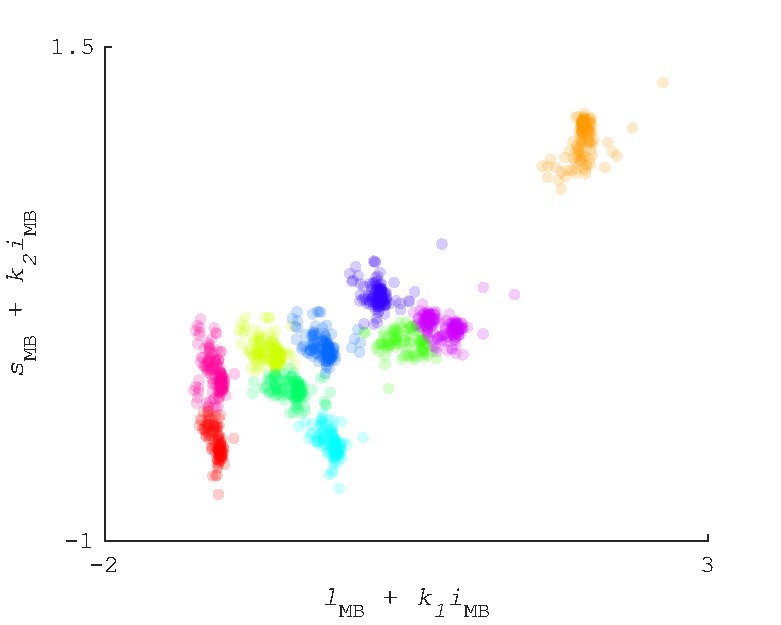
\includegraphics[max width=\textwidth]{figs/comp/KMeansMarkDemo/1.pdf}
 \caption{A reproduction of Figure \ref{fig:KM1} from Page \pageref{fig:KM1}, which shows the results of a k-means clustering of the data from Figure \ref{fig:corrected} from Page \pageref{fig:corrected} (which shows the \emph{actual} groups.}
 \label{fig:KM1lr}
\end{figure} 

The standard algorithm proceeds as follows: 

\begin{enumerate}
    \item $k$ random starting positions are assigned. 
    \item Each data-point is assigned a group based on which starting position is closest.
    \item The mean location of the data-points in each group is computed.
    \item Steps 2 and 3 are repeated, using the computed means instead of the original starting positions, until a stage where an iteration of these two steps results in no data-point changing groups. Once this occurs, the algorithm is said to have converged, and the resulting groupings are output.
\end{enumerate}

\subsection{Principal Component Analysis}

\textit{A valuable primer on \acrshort{PCA} in relation to colour technology is available from \citet{tzeng_review_2005}.}

\bigskip

\glsreset{PCA}
\Gls{PCA} is a dimensionality reduction method, used to to reduce the number of variables within a dataset whilst retaining as much of the variance as possible, and often used to identify the correlated roots of variance.

\begin{figure}[htbp]
 \includegraphics[max width=\textwidth]{figs/LitRev/PCA.png}
 \caption{Two-dimesional data with the first and second principal components added. Source: \url{https://commons.wikimedia.org/wiki/File:GaussianScatterPCA.svg}}
 \label{fig:PCA}
\end{figure} 

Along with similar techniques (such as single value decomposotion), it is used extensively within the study of daylight \glspl{SPD} \citep{hernandez-andres_color_2001,ojeda_influence_2012,pant_estimating_2009,bui_group_2004,judd_spectral_1964,maloney_computational_1984,spitschan_variation_2016} and natural \glspl{SRF} \citep{maloney_computational_1984,dzmura_color_1992,maloney_evaluation_1986,maloney_color_1986,cohen_dependency_1964,ferrero_principal_2011,zhang_reconstructing_2008,kwon_surface_2007,agahian_reconstruction_2008,harifi_recovery_2008,parkkinen_characteristic_1989,vrhel_color_1992,fairman_principal_2004,ayala_use_2006,eem_reconstruction_1994-2,connah_multispectral_2006,shi_using_2002,morovic_metamer-set-based_2006}. 

%A key goal for many of the researchers listed above... - how many dimensions/sensors do we need

In eras where the transmission of large datasets was troublesome, dimensionality reduction methods such as \gls{PCA} held value as a method to summarise a dataset, with the understanding that a reader could reconstruct a pseudo-dataset with minimal data-loss from the provided principal components. One such example is the work of \citet{judd_spectral_1964} where only the mean and first four characteristic vectors are provided\footnote{This is not technically \gls{PCA} but the related technique of \citet{morris_objective_1954}.}. The data from this study is replotted in Figure \ref{fig:Judd} and it can be seen that for their dataset this description does seem to offer a sensible summary of the data: the shape of the mean can be seen, and it can be seen that further variation principally occurs as a result of $V_{2}$ which is a broad and relatively monotonic function, indicating that changes are likely to be a skewing of the spectral shape.

\begin{figure}[htbp]
 \includegraphics[max width=\textwidth]{figs/LitRev/Judd.pdf}
 \caption{The mean and first four characteristic vectors of \citet{judd_spectral_1964}.}
 \label{fig:Judd}
\end{figure} 

\section{Interim Summary}

This chapter has laid out the most relevant developments in the research areas which the other chapters of this thesis build upon. 

Chapter \ref{chap:Interviews} builds upon our museum lighting knowledge by filling the gap in our understanding of how museum lighting is actually thought about and selected currently, and tries to identify the most fruitful avenue for future research which will allow the reduction of damage to objects in museums.

Chapters \ref{chap:LargeSphere} and \ref{chap:SmallSphere} target the interaction between colour constancy and \glspl{ipRGC}, using some of the methodologies covered in the Section \ref{sec:methodsforCC} and the knowledge of the physiology of \glspl{ipRGC} outlined in Section \ref{sec:ipRGCs} to build upon the experiments summarised in Section \ref{sec:ipRGCbeyond}.

Chapter \ref{chap:Tablet} investigates a new methodology (a variant of achromatic setting, described in Section \ref{sec:methodsforCC}) for performing colour constancy experiments, using museum spaces as test spaces due to their well controlled lighting environments.

Chapter \ref{chap:Melcomp} takes a more theoretical look at the relationship between colour constancy and \glspl{ipRGC} using a computational methodology, and the mathematical methods described in Section \ref{sec:math}.
